\documentclass[10pt]{scrartcl}

\usepackage[utf8]{inputenc}
\usepackage{tabularx}
\usepackage[ngerman]{babel}
\usepackage[automark]{scrpage2}
\usepackage{amsmath,amssymb,amstext}
%\usepackage{mathtools}
\usepackage[]{color}
\usepackage[]{enumerate}
\usepackage{graphicx}
\usepackage{lastpage}
\usepackage[perpage,para,symbol*]{footmisc}
\usepackage{listings} 
\usepackage[pdfborder={0 0 0},colorlinks=false]{hyperref}
\usepackage[numbers,square]{natbib}
\usepackage{color}
\usepackage{colortbl}
\usepackage{listings}
\usepackage{a4wide}
\usepackage{xspace}
\usepackage{listings}
\usepackage{hyperref}
\usepackage{epstopdf}

\lstset{numbers=left, numberstyle=\tiny, numbersep=5pt, breaklines=true, showstringspaces=false} 

%changehere
\def\titletext{TH1 Praktikum 3 : Ausarbeitung}
\def\titletextshort{Praktikum 3}
\author{Carsten Noetzel, Armin Steudte}

\title{\titletext}

%changehere Datum der Übung
\date{16.05.2012}

\pagestyle{scrheadings}
%changehere
\ihead{TH1, Padberg}
\ifoot{Generiert am:\\ \today}

\cfoot{Carsten Noetzel, Armin Steudte}


\ohead[]{\titletextshort}
\ofoot[]{{\thepage} / \pageref{LastPage}}

\setlength{\parindent}{0.0in}
\setlength{\parskip}{0.1in}

\begin{document}
\maketitle

\setcounter{tocdepth}{3}
\tableofcontents
\listoffigures
%\lstlistoflistings

\section{Aufgabe 1}
\begin{enumerate}
\item{Reversibilität / Lebendigkeit}\\
Lebendigkeit $\Rightarrow$ Reversibilität, da aus der Lebendigkeit folgt, dass es eine echt positive T-Invariante gibt für die gilt $\forall t \in T : I_{T}(t) \geq 1$. Weiterhin setzt ein lebendiges Netz voraus, dass alle $t \in T$  M-aktiviert sind, wodurch man von einer beliebigen Markierung M aus jede Transition erreichen können muss.\\
Die Umkehrung gilt nicht! Reversibilität $\nRightarrow$ Lebendigkeit

\item{Beschränktheit / Lebendigkeit}\\
Zwischen der Beschränktheit eines Netzes und seiner Lebendigkeit gibt es keinen direkten Zusammenhang. Ein Netz kann beschränkt und lebendig (Abbildung \ref{fig:BL}), beschränkt und nicht lebendig (Abbildung \ref{fig:BnL}), unbeschränkt und lebendig (Abbildung \ref{fig:nBL}) und unbeschränkt und nicht lebendig sein (Abbildung \ref{fig:nBnL}).

\begin{figure}
\begin{minipage}[hbt]{7cm}
	\centering
	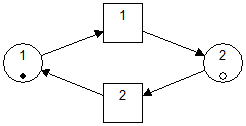
\includegraphics[width=0.7\textwidth]{Bilder/2_Beschraenkt_und_Lebendig.png}
	\caption{beschränktes und lebendiges Netz}
	\label{fig:BL}
\end{minipage}
\hfill
\begin{minipage}[hbt]{7cm}
	\centering
	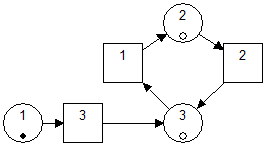
\includegraphics[width=0.7\textwidth]{Bilder/2_Beschraenkt_nicht_Lebendig.png}
	\caption{beschränktes und nicht lebendiges Netz}
	\label{fig:BnL}
\end{minipage}
\end{figure}
\begin{figure}
\begin{minipage}[hbt]{7cm}
	\centering
	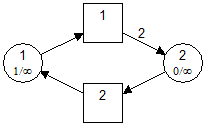
\includegraphics[width=0.7\textwidth]{Bilder/2_Nicht_Beschraenkt_und_Lebendig.png}
	\caption{unbeschränktes und lebendiges Netz}
	\label{fig:nBL}
\end{minipage}
\hfill
\begin{minipage}[hbt]{7cm}
	\centering
	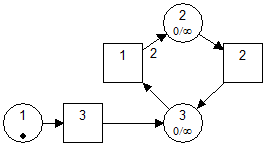
\includegraphics[width=0.7\textwidth]{Bilder/2_Nicht_Beschraenkt_nicht_Lebendig.png}
	\caption{unbeschränktes und nicht lebendiges Netz}
	\label{fig:nBnL}
\end{minipage}
\end{figure}

\item{Beschränktheit / Reversibilität}\\
Zwischen Beschränktheit und Reversibilität eines Netzes gibt es keinen direkten Zusammenhang. Ein Netz kann beschränkt und reversibel (Abbildung \ref{fig:BR}), beschränkt und nicht reversibel (Abbildung \ref{fig:BnR}), unbeschränkt und reversibel (Abbildung \ref{fig:nBR}) und unbeschränkt und nicht reversibel sein (Abbildung \ref{fig:nBnR}).


\begin{figure}
\begin{minipage}[hbt]{7cm}
	\centering
	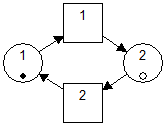
\includegraphics[width=0.7\textwidth]{Bilder/3_beschraenkt_und_reversibel.png}
	\caption{beschränktes und reversibles Netz}
	\label{fig:BR}
\end{minipage}
\hfill
\begin{minipage}[hbt]{7cm}
	\centering
	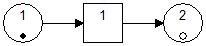
\includegraphics[width=0.7\textwidth]{Bilder/3_beschraenkt_nicht_reversibel.png}
	\caption{beschränktes und nicht reversibles Netz}
	\label{fig:BnR}
\end{minipage}
\end{figure}
\begin{figure}
\begin{minipage}[hbt]{7cm}
	\centering
	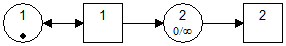
\includegraphics[width=0.7\textwidth]{Bilder/3_unbeschraenkt_und_reversibel.png}
	\caption{unbeschränktes und reversibles Netz}
	\label{fig:nBR}
\end{minipage}
\hfill
\begin{minipage}[hbt]{7cm}
	\centering
	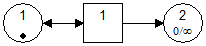
\includegraphics[width=0.7\textwidth]{Bilder/3_unbeschraenkt_nicht_reversibel.png}
	\caption{unbeschränktes und nicht reversibles Netz}
	\label{fig:nBnR}
\end{minipage}
\end{figure}

\item{Erreichbarkeit / Lebendigkeit}\\
Lebendigkeit $\Rightarrow$ Erreichbarkeit\\
Wenn ein $t \in T$ lebendig ist, muss es $\forall M \in EG$ M-erreichbar sein, daraus folgt $\exists M \in EG$ für das gilt t ist aus M erreichbar.\\
Wenn das Netz lebendig ist, sind alle Transitionen lebendig und damit $\forall M \in EG$ M-erreichbar.

\item{Erreichbarkeit / Reversibilität}\\
Reversibilität $\Rightarrow$ Erreichbarkeit\\
Wenn ein Netz reversibel ist, muss es einen Weg von $M_{0} \overset{*}{\rightarrow} M \overset{*}{\rightarrow} M_{0}$ geben, somit gilt: $\forall t \in T$ sind von jeder $M \in EG$ M-erreichbar.
Die Umkehrung gilt nicht! Erreichbarkeit $\nRightarrow$ Reversibilität

\item{Erreichbarkeit / Beschränktheit}\\
\label{erreichbarkeit_beschraenktheit}
Es gibt keinen Zusammenhang. Da die Erreichbarkeit $\forall t \in T$ ein notwendiges Kriterium dafür ist, dass ein Netz lebendig ist, kann an dieser Stelle auf die Beispiele aus Punkt 2 verwiesen werden.\\
Ein Netz kann beschränkt sein und alle $t \in T$ sind erreichbar (lebendig) (Abbildung \ref{fig:BL}), beschränkt und nicht alle $t \in T$ sind erreichbar (nicht lebendig) (Abbildung \ref{fig:BnL}), unbeschränkt und alle $t \in T$ sind erreichbar (lebendig) (Abbildung \ref{fig:nBL}) und unbeschränkt und nicht alle $t \in T$ sind erreichbar (nicht lebendig) sein (Abbildung \ref{fig:nBnL}).

\item{Stelleninvarianten / Lebendigkeit}\\
Stelleninvarianten sagen etwas über die Beschränktheit von Netzen aus. Da bereits gezeigt wurde, dass es keinen Zusammenhang zwischen Beschränktheit und Lebendigkeit gibt, sei hier auf die Beispiele aus Punkt 2 verwiesen.\\
Für die beschränkten Netze aus Abbildung \ref{fig:BL} und \ref{fig:BnL} gibt es Stelleninvarianten, für die unbeschränkten Netze aus Abbildung \ref{fig:nBL} und \ref{fig:nBnL} gibt es keine Stelleninvarianten unabhängig davon ob das Netz lebendig ist oder nicht.

\item{Stelleninvarianten / Reversibilität}\\
Es gibt keinen direkten Zusammenhang. Gibt es keine Stelleninvariante ist das Netz unbeschränkt und kann sowohl reversibel als auch nicht reversibel sein. Hierzu sei auf die Beispiele von Punkt 3 verwiesen.

\item{Stelleninvarianten / Beschränktheit}\\
$\forall p \in P$ $I_{P}(p) > 0$ und $I_{P}(p')\geq 0$ $\forall p' \in P$ $\Rightarrow$ p ist beschränkt\\
Gehören alle $p \in P$ einer solchen positiven Stelleninvariante an $\Rightarrow$ Netz ist beschränkt\\
Die Umkehrung gilt nicht! Beschränktheit $\nRightarrow$ $\forall p \in P$ gehören positiver Stelleninvariante an

\item{Stelleninvarianten / Erreichbarkeit}\\
Die Stelleninvariante trifft Aussagen bezüglich der Beschränktheit eines Netzes.
Wie bereits unter dem Punkt \ref{erreichbarkeit_beschraenktheit} diskutiert wurde, existiert zwischen Beschränktheit und Erreichbarkeit kein direkter Zusammenhang.
Hierbei sei auch auf die unter dem Punkt referenzierten Beispiele verwiesen.

\item{Transitionsinvarianten / Lebendigkeit}\\
Zwischen der Transitionsinvariante und Lebendigkeit existiert der Zusammenhang, dass Lebendigkeit $\Rightarrow$ pos. Transitionsinvariante.\\
Da $N_{M0}$ lebendig ist, wenn $\forall t \in T$ lebendig sind.
Eine Transition $t \in T$ ist lebendig, wenn sie für alle $M \in EG$ M-erreichbar ist.
Somit beschreibt die Transitionsinvariante den Zyklus, dass wenn $t$ geschaltet hat es durch geforderte M-Rrreichbarkeit auch wieder schalten kann. 

\item{Transitionsinvarianten / Reversibilität}\\
Wenn $N_{M0}$ reversibel ist $\exists$ T-Invariante, da es einen Zyklus von $M_{0} \overset{*}{\rightarrow} M  \overset{*}{\rightarrow} M_{0}  \forall M \in EG$ für Reversibilität geben muss.

\item{Transitionsinvarianten / Beschränktheit}\\
Die Beschränktheit stellt eine notwendige Bedingung für das Vorliegen einer Transitionsinvariante dar.
Ohne Beschränktheit kann es kein Transitionsinvariante geben, da man von einem beliebigen Markierung dann nicht mehr zur gleichen Markierung im EG zurückkommen kann.
Es existiert damit keine Schaltsequenz $M \overset{*}{\rightarrow} M$.

\item{Transitionsinvarianten / Erreichbarkeit}\\
Wie bereits erwähnt folgt aus Lebendigkeit $\Rightarrow$ pos. Transitionsinvariante und Lebendigkeit $\Rightarrow$ Erreichbarkeit. 
Da für die Lebendigkeit eines Netzes $N_{M0}$ M-Erreichbarkeit $\forall t \in T$ vorausgesetzt wird und aus Lebendigkeit auf das Vorhandensein einer pos. Transitionsinvariante geschlossen werden kann gilt: Positive Transitionsinvariante $\Leftarrow$ Lebendigkeit $\Rightarrow$ Erreichbarkeit.

\item{Transitionsinvarianten / Stelleninvarianten}\\
Damit eine Transitionsinvariante existieren kann muss das Netzt $N$ mindestens aus einer Transition und einer Stelle bestehen (die Stelle $p_{1}$ stellt die Vor- und Nachbedingung von $t_{1}$ in diesem Fall dar, $\bullet t_{1} = \{p_{1}\}$ und $t_{1} \bullet = \{p_{1}\}$ ).\\
Da mit dem Vorhandensein einer Stelle auch eine Stelleninvariante existiert gilt: $\exists Transitionsinvariante \Rightarrow \exists Stelleninvariante$

\item{Überdeckungsgraph / Lebendigkeit}\\
Lebendigkeit baut auf dem EG auf. Ist eine Transition $t \in T$ im EG M-erreichbar, so ist sie auch im UG M-erreichbar.
Somit ist ein Netz $N$ welches im EG lebendig ist auch im UG lebendig.

\item{Überdeckungsgraph / Reversibilität}\\
$\exists \omega$-Markierung im UG $\Rightarrow$ EG ist unendlich $\Rightarrow$ Netz ist nicht reversibel, da keine Schaltsequenz $M_{0} \overset{*}{\rightarrow} M_{0}$ existiert.

\item{Überdeckungsgraph / Beschränktheit}\\
Sind UG und EG identische (keine $\omega$-Markierungen im UG) $\Rightarrow$ das Netz $N$ ist beschränkt.
$\exists \omega$-Markierung im UG $\Rightarrow$ Netz $N$ ist unbeschränkt.

\item{Überdeckungsgraph / Erreichbarkeit}\\
Ist eine Transition im EG M-erreichbar, so ist sie auch im UG M-erreichbar. $\exists M \in EG \Rightarrow M \in UG$ ggf. überdeckt durch $\omega$-Markierung.

\item{Überdeckungsgraph / Stelleninvarianten}\\
$\exists$ P-Invariante dann ist das Netz $N$ beschränkt. 
Wenn das Netz beschränkt ist sind EG und UG identisch.
Das bedeutet: $\exists$ P-Invariante $\Rightarrow$ EG=UG.

\item{Überdeckungsgraph / Transitionsinvarianten}\\
$\exists$ T-Invariante so gibt es einen Zyklus EG.
Somit existiert dieser Zyklus auch im UG.

\item{Kondensation des EG / Lebendigkeit}\\
\label{eg_lebendigkeit}
Besitz der KG des EG mehr als einen Knoten so ist das Netz nicht lebendig, da die Transition t, die zwischen zwei Knoten im Kg schaltet, nicht M-erreichbar ist.\\
Somit kann die Bedingung für Lebendigkeit ($\forall t \in T$, $t$ ist M-erreichbar) nicht erfüllt sein.

\item{Kondensation des EG  / Reversibilität}\\
Besitzt eine KG mehr als einen Knoten $\Rightarrow$ das Netz $N$ ist nicht reversibel, da ein Reversibles Netz von jeder Markierung M im EG nach $M_{0}$ schalten kann und somit zu einem Knoten im KG zusammenfällt. 

\item{Kondensation des EG  / Beschränktheit}\\
Um einen KG aufbauen zu können muss das Netz beschränkt sein. 
Der EG eines unbeschränkten Netzes ist unendlich, wodurch sich kein KG erstellen lässt. 

\item{Kondensation des EG  / Erreichbarkeit}\\
KG hat mehr als einen Knoten $\Rightarrow$ nicht alle $t \in T$ sind M-erreichbar (vgl. \ref{eg_lebendigkeit}).

\item{Kondensation des EG  / Stelleninvarianten}\\

\item{Kondensation des EG  / Transitionsinvarianten}\\

\item{Kondensation des EG  / Überdeckungsgraph}\\

\item{Verklemmung / Lebendigkeit}\\

\item{Verklemmung / Reversibilität}\\

\item{Verklemmung / Beschränktheit}\\

\item{Verklemmung / Erreichbarkeit}\\

\item{Verklemmung / Stelleninvarianten}\\

\item{Verklemmung / Transitionsinvarianten}\\

\item{Verklemmung / Überdeckungsgraph}\\

\item{Verklemmung / Kondensation des EG}\\

\end{enumerate}
\textbf{Reversibilität / Lebendigkeit}


\section{Aufgabe 2}

\end{document}

